\documentclass{article}
\usepackage{fullpage}
\usepackage[czech]{babel}
\usepackage{amsfonts}
\usepackage{graphicx}
\usepackage{caption}
\usepackage{mhchem}
\graphicspath{{images/}}

\title{\vspace{-2cm}Organická chemie\vspace{-1.7cm}}
\date{}
\author{}

\begin{document}
\maketitle

\begin{itemize}
  \item věda, který se zabývá studiem struktury, vlasností, přípravou a použitím organických sloučenin
  \item je to chemie sloučenin uhlíku s biogenními prvky - vodíkem, kyslíkem, dusíkem, sírou, fosforem, hoříček, vápníkem
  \item základní vlastnost uhíku v organických sloučeninách = čtyřvaznost, důvodem je hybridizace - sjednocení energeticky různých orbitalů daného atomu, přičemž vznikají nové orbitaly, tzv. orbitaly hybridní
  \item prvně středověk - \textbf{Paracelsus} - doktoři jsou na to, aby míchali léky - iatrochemie (16. st.)
  \item pak novověk - \textbf{Berzelius} - živočišné a rostlinné sloučeniny vznikají jenom díky ,,životní síle" (vis vitalis) - tzv. \textit{vitalistická teorie} (18. st.), tato brzo vyvrácena r. 1828 \textbf{F. Wöhlerem}, který v laboratoři z anorg. látky vytvořil org. látku močovinu
  \item na konci 19. st. průkopník \textbf{F. A. Kekulé} - definoval, že chemické vlasnosti organických sloučenin souvisí s jejich vnitřní stavbou, pak definoval několik základních postulátu, které platí dodnes
  \begin{itemize}
    \item uhlík je vždy čtyřvazný - z uhlíku vždycky vychází čtyři vazby
    \item všechny čtyři vazby atomu uhlíku jsou rovnocenné - důvodem je \textit{hybridizace} - viz dále
    AAAAAAAAA OBRÁZEK ZÁKLADNÍ STAV, EXCITOVANÝ STAV
    \item uhlíkové atomy mají schopnost vytvářet řetězce otevřené i uzavřené (tedy i cyklické)
    \item atomy jsou v nich vázány jednoduchými, dvojnými, nebo trojnými vazbami (vždy tedy tak, aby z jednoho uhlíku vycházely dohromady čtyři vazby)
  \end{itemize}
  \item hybridizace
  \begin{itemize}
    \item proces sjednocení energeticky různých orbitalů daného atomu, přičemž vznikají nové orbitaly, tzv. \textit{hybridní orbitaly}
    \item typy hybridizace:
    \begin{itemize}
      \item úplná - sp3 - čtyři stejné vazby, každá sigma - do tetraedru
      \item částečná trigonaální - sp2 trojúhelníková 120 stupnů - jedna dvojna (sigma, pi), dve jednoduche
      \item částečná lineární - sp lineární 180 stupnu, jedna trojna (sigma, dve pi), jedna jednoducha
    \end{itemize}

  \end{itemize}
  \item klasifikace uhlovodíků
  \begin{itemize}
    \item acyklické
    \begin{itemize}
      \item nasycené - všechny vazby jednoduché
      \item nenasycené - ne všechny vazby jednoduché
    \end{itemize}
    \item cyklické
    nedavam AAAAAAAAAAAA DODĚLAT
    stereochemie - zabývá se strukturou látek, nauka o prostorovém uspořádání atomů v molekule
    konstituce a konfigurace
      konstituce - řazení atomů za sebou
      konfigurace - umístění atomů v prostoru
    názvosloví - NAPROSTO DEBILNÍ
  \end{itemize}
  \item reakce organických látek
  \begin{itemize}
    \item bývají pomalejší než anorganické, mají složitjší průběh
    \item nevyrovnáváme, protože bysme se nedopočítali
    \item základní typy
    \begin{itemize}
      \item podle způsobu štěpení vazby
      \begin{itemize}
        \item homolýza - rovnoměrné, symetrické štěpení, vnikají radikály - částice s jedním volným nepárovným elektronem
        \item heterolýza - nerovnoměrné, nesymetrické štěpení, vznik nových, el. nabitých částic - jedna část si odtáhne elektrony, jedna ne
      \end{itemize}
      \item podle charakteru částic v reakci
      \begin{itemize}
        \item elektrofilní - vzniklé částice vyhledávají záporný náboj (vyhledávají přebytek elektronů), tedy jsou kladně nabité, např $H^+$
        \item nukleofilní - částice vyhledávají kladný náboj (mají přebytek elektronů), tedy jsou záporně nabité, např. $OH^-$
        \item radikálové - částice nesoucí nepárový elektron, velice reaktivní
      \end{itemize}
      \item podle celkové změny na substrátu - na tom, co vchází do reakce
      \begin{itemize}
        \item substituce = nahrazování = zaměňování - dochází k náhradě jednoho nebo více atomů (jedné nebo více atom. skupin) substrátu jiným atomem nebo skupinou atomů
        ite
        \begin{enumerate}
          \item radikálová - dochází k homolytickému štěpení pomocí radikálů, má tři fáze
            \begin{enumerate}
              \item iniciace - jde nám o vznik radikálů
              \item propagace - jde nám o samotnou reakci
              \item terminace - jde nám o zánik radikálů a o izolaci produktů
            \end{enumerate}
            \item elektrofilní - reakce s elektrofilním činidlem, které vzniká v průběhu reakce, např. nitrace benzenu
            \item nukleofilní - nukleofilní činidlo reaguje s uhlíkovým atomem s částečně kladným nábojem
        \end{enumerate}
        \item eliminace = odštěpení = odejmutí - děj, při kterém se uvolňuje molekula jednoduché, většinou anorganiceké látky, kvůli čemuž vzniká v molekule substrátu násobná vazba, nebo se zvyšuje její násobnost
        \begin{enumerate}
          \item dehydratace - osštěpují se molekuly vody
          \item dehdrogenace - odštěpují se atomy vodíku
          \item dehydrohalogenace - odštěpují se molekuly halogenovodíků
        \end{enumerate}
        \item adice = připojení = opak eliminace - vecpeme tam molekulu, snížíme násobnost vazby
        \begin{enumerate}
          \item elektrofilní - elektrofilní činidlo reaguje s pi-elektrony násobných vazeb uhlíku
          \item nukleofilní - nukleofilní činidlo se aduje na uhlík ve vazbě nesoucí částečný kladný náboj, probíhají na dvoujnou vazbu C=O
        \end{enumerate}
        \item molekulový přesmyk = isomerace, reakce v jejímž průběhu dochází k přesunu (přeskupení) určitých atomů z jednoho místa v molekule na místo jiné, aniž se měni chemické složení (souhrnný vzorec) v dané sloučenině
      \end{itemize}
    \end{itemize}
    \item v organice najdeme i běžné redoxní a acidobazické reakce
  \end{itemize}
  \item zápis reakce
  \begin{itemize}
    \item reakční schéma - zjednodušený zápis reakce: suroviny $\rightarrow$ produkty OBRAZEKOBRAZEK
    \item reakční mechanismus - podrobný popis přeměny výchozích látek na produkty včetně popisu všech meziproduktů OBRAZEKOBRAZEK
  \end{itemize}
  \item pravidla pojmenovávání org. sloučenin
  \begin{itemize}
    \item viz obrázek OBRAZEKOBRAZEK na discordu
    \item začínáme nasycenými uhlovodíky - alkany
    \begin{itemize}
      \item musíme najít tzv. základní hybrid - nejdelší řetězec, nejvíce násobných vazeb a nejvíce vedlejších řetězců - substituentů a pojmenuju ho podle počtu uhlíků (níže) s příponou -an
      \item tento pak očísluju ze směru, kde mám dříve substituent (když jsou substituenty stejně, tak porovnávám druhé substituenty, třetí substituenty, ...) a substituenty taky pojmenuju podle počtu uhlíků, ale přípona je -yl, před ně ještě přidám číslovku uhlíku základního hydridu - lokantu, na který je připojený, když je jich více stejných tak čísla dávám za sebe, odděluju čárkou a píšu di-,tri-,...
      \item pak to spojuju pomlčkama, substituenty seřazuju podle abecedy (příčemž ignoruju předpony di-, tri-, ..., cyklo-, takže např. 1-ethyl-1,2-dimethyl), mezi posledním substituentem a názvem základního hydridu pomlčka není, takže např. 4-ethyl-3-methylhexan
      \item když mám někde cyklickou část, tak to porovnám s normálním základním hydridem, a hlavní bude ten, který je delší, před název cyklické části dám cyklo- a číslování bude zase takové, aby součet čísel lokantů se substituenty byl co nejmenší (ekvivalentní s pravidlem pro necyklické uhlovodíky), takže např. 4-ethyl-1,1,2-trimethylcyklohexan, když je to jako substituent tak zase cyklo-[]-yl
      \item můžeme mít uhlovodík s nějakou volnou vazbou, že se od něj něco odtrhlo (on se od něčeho odtrhl), pak názvosloví funguje pořád stejně, ale představím si tu volnou vazbu jako substituent beze jména, tedy jen číslo lokantu a -yl a toto napíšu až nakonec, za jméno hlavního řetězce, takže např. propan-2-yl; popř. si můžu vybrat základní řetězec tak, aby na té volné vazbě začínal, pak i hlavní řetězec nazvu jako -yl (ne jako -an) a číslo vynechám (protože tedy vždy 1), takže např. 1-methylethyl, btw vždycky dávám v číslování přednost volné vazbě před ostatníma srandárnama
      \item když to všecho poskládám - když mám větvený substituent tak tu vazbu, kterou se připojuje na hlavní hydrid beru jako volnou, podle toho taky pojmenovávám, pak to poskládám dohromady, názvy substituentů ve větveném substituentu se řadí absolutně podle abecedy (včetně di-, tri-, ..., cyklo-), toto všechno dám do závorky a už se k tomu chovám jako k normálnímu názvu (před to číslo lokantu hl. hydridu, pomlčku, po něm pomlčku, popř. jestli je to jako poslední substituent tak po něm nenapíšu pomlčku)
      \item názvy podle počtu uhlíků
      \begin{itemize}
        \item meth -
        \item eth  -
        \item prop -
        \item but -
        \item pent -
        \item hex
        \item hept
        \item okt
        \item non
        \item dek
        \item undek
        \item dodek
        ...
        \item ikos
        ...
        \item triakont
      \end{itemize}
    \end{itemize}
  \end{itemize}
\end{itemize}

AAAAAAA 22.3.2023 HOMOLOGICKÁ ŘADA, ALKANY, ALKENY
\begin{itemize}
  \item uhlovodíkový zbytek, který má dvě volné vazby má koncovku -ylen
  6-methyl-3-cyklopropyldekan
  1-ethyl-2-methyl-1,3-dipropylcyklopentan
  1-cyklobutyl-4-(propan-2-yl)cyklohexan
\end{itemize}
výskyt alkanů
\begin{itemize}
  \item v atmosféře - nepatrné množství methanu - vzniká činností methanogenních bakterií (nejen) v travicích soustavách
  \item nejpodstatnější složka zemního plynu
  \item nižší kapalné alkany - v silicích vyšších rostlin
  \item vyší pevné alkany - živočichové
\end{itemize}
vlastnosti
\begin{itemize}
  \item s vyšším počtem uhlíků rostě skupenství (plyn - kap - pev) a teplota tání a varu
  \item jsou málo reaktivní -- nascené, slouhé sigma vazby
  \item reakce alkanů
  \begin{itemize}
    \item radikálová substituce - musíme vyrobit radikály, ty pak reagují (např. s chlorem -- chlorace)
    \begin{itemize}
      \item iniciace -- vznik radikálů
      \item propagace -- vlastní průběh reakce, radikál odtrhne jeden vodík (wow), vzniká methylový radikál, tento reaguje s dalším neradikálem ze kterého vzniknce další radikál, toto dokola
      \item terminace -- zánik radikálu, většinou tak, že se všechny spotřebují a zreagují s něčím, vzniká směs různých produktů (např. u chlorace vznikají v poměru chlormethan $CH_3Cl$, methylchlorid $CH_2Cl_2$, trichloromethan (chloroform) $CHCl_3$, tetrachlormethan $CCl_4$)
    \end{itemize}
  \end{itemize}
\end{itemize}

nevim vole příklady
2,3,3,4-tetramethylheptan
4-ethyl-2-methylhexan
3-ethyl-3-methylpentan
4,4-diethyl-5-methyloktan

\begin{itemize}
  \item idk co za nadpis -- Nenasycené uhlovodíky
  \item tedy ne všechny vazby jsou jednoduché, mám dvojné, trojné vazby
  \item dvojná vazba -- koncovka -en (-dien, -trien, ...) -- alkeny (alkadieny, alkatrieny, ...)
  \item trojná vazba -- koncovka -yn -- alkyny
  \item taky mohou být cyklycké řetězce -- předpona cyklo-
  \item potom tedy základ názvu (meth, eth, prop, ...), pomlčka, číslo lokantu, ze kterého vychází dvojná vazba, pomlčka a koncovka, tedy např. but-2-en, čísluju tak, aby dvojná vazba měla co nejnižší číslo lokantu
  \item např. 2-methyl-but\textbf{a}-1,3-dien (a protože čeština údajně)
  \item když máme vazbu dojnou i trojnou, tak u číslování upřednostňujeme dvojnou vazbu, píšeme ale prvně dvojné vazby, pak trojné, tedy např. but-1-en-3-yn, okta-1,4-dien-7-yn, 5-butyl-hepta-1,3,6-trien
  \item když máme volnou vazbu, má přednost před dvojnou vazbou a pak to napíšeme na konci, tedy např. but-3-en-1-yl
  \item můžeme mít dvojnou vazbu v cyklu, tedy např. 3-ethylcyklohex-1-en, 3-ethyl-4-methylcyklopent-1-en, 5-propylcyklohexa-1,3-dien
  \item tedy např. 8-methylcyklookta-1,3,6-trien, buta-1,2-dien, 2-methylbuta-1,3-dien
\end{itemize}

\subsection{Reakce alkenů}
\begin{itemize}
  \item MOC TOHO CHYBÍ AAAAAAAAAAA -- adice (kys. a vody, halegonů, oxidace, hydrogenace)
\end{itemize}

\subsubsection{Polymerace}
\begin{itemize}
  \item mer = jednotka, polymer = více jednotek
  \item např. ethen se teplem polymeruje -- dvojná vazba se zjednotí, druhou se chytne dalšího ethenu $\rightarrow$ polymer OBRAZEKOBRAZEK
\end{itemize}

jsou tři typy alkadienů podle postavení dojné vazby -- kumulované (obě vazby z jednoho uhlíku, dost nestabilní, dv. vazb. se hodně ovlivňují), konjugované (mezi dv. vazb. je jedna jednoduchá vazba, stabilnější, dv. vazb. se ovlivňují míň) a isolované (dv. vazb. dál od sebe, už se neovlivňují, nejstabilnější)

\subsection{Zástpuci alkenů}
\begin{itemize}
  \item ethylen
  \item popylen $\rightarrow$ polymerace
  \item buta-1,3-dien -- výroba syntetického kaučuku
\end{itemize}

\section{Alkyny}
\begin{itemize}
  \item trojná vazba
  \item jedna sigma, dvě pí vazby
  \item jsou mírně kyselé, protože dokážou disociaovat (?) H+
  \item reakce obdobně jako u alkenů
  \begin{itemize}
    \item adice halogenů --  OBRAZEKOBRAZEK, HO2CC- - - CCO2h + Br2 -> reaguje
    \item adice nukleofilní -- kučerovova reakce
    \item oxidace -- sloučeniny s dvojnou a trojnou vazbou oxidují snadno
  \end{itemize}
  \item zástupci
  \begin{itemize}
    \item acetylen -- bezbarvý plyn, se vzduchem tvoří výbušnou směs, výroba: CaC2 + 3H20 -> C2H2 + Ca(OH)2, využíán k autogennímu svařování -- tvoří plamen o teplotě až 3000 stupňů C; OBRAZEKOBRAZEK
  \end{itemize}
\end{itemize}

\section{Aromatické sloučeniny}
\begin{itemize}
  \item areny, mají vůni -- aroma
  \item základem je benzen -- $C_6H_6$ OBRAZEKOBRAZEK, ten má atypický řád vazby 1,5 (ani jednoduchá ani dvojná), má el. hustotu nad a pod základním skeletem -- el. jsou tzv. delokalizované OBRAZEKOBRAZEK
  \item jsou areny monocyklické i polycyklické (více spojených benzenů), v polycyklických arenech jádra isolovaná (oddělená alespoň jednou vazbou, např. bifenyl, pozor na číslování (viz obrázek) OBRAZEKOBRAZEK I S CISLOVANIM) nebo kondensovaná (jádra napojena přímo na sebe, např. naftalen, anthracen, pozor na číslování (viz obrázek) OBRAZEKOBRAZEK I S CISLOVANIM)
  \item názvosloví (pomoc)
  \begin{itemize}
    \item vychází z triviálních názvů základních aromátů a přidávají se předpony, tedy např. methylbenzen (trivialně toluen), 1,2-dimethylbenzen (pozor, protože cyklické tak nemá smysl číslovat benzen, tj. číslujeme substituenty dle pozice mezi sebou -- 1,2 bude ortho, zkratka o-; trivialně o-xylen), 1,3-dimethylbenzen (1,3 -- meta, m-; trivialně m-xylen), 1,4-dimethylbenzen (1,4 -- para, p-; trivialně p-xylen)
    \item benzen s jednou volnou vazbou se trivialně nazývá fenyl, s jedním uhíkem navíc a volnou jednoduchou vazbou benzyl, s jedním uhlíkem navíc a volnou dvojnou vazbou benzyliden, s jedním uhlíkem navíc a volnou trojnou vazbou benzylidyl
    \item monocyklické areny můžu většinou pojmenovat asi na čtyřikrát, podle toho kterou část vezmu jako základní, tedy např. 2-methylbenzen-1-yl, 2-methylfenyl, 2-tolyl, o-tolyl
  \end{itemize}
  \item typy
  \begin{itemize}
    \item monocyklické -- jeden cyklus, nepolární, kapalné a tuhé, body varu rostou se zvyšujícím se počtem uhlíků
    \item vícejaderné -- více uhlíků, tuhé, některé karcinogenní
  \end{itemize}
  \item reakce
  \begin{itemize}
    \item nejčastěji elektrofilní substituce -- na každém z uhlíků benzenu je navázaný vodík, což je elektrofil, takže positivní substituenty se dají zaměnit za vodík
    \item typy elektrof. subs.
    \begin{itemize}
      \item halogenace -- elektrof. činidlem halogen, potřebujeme katalyzátor ve formě Lewisovské kyseliny, výsledkem chlorbenzen, brombenzen
      \item nitrace -- elektrof. částicí nitroniový kation $NO_2^+$, který je tvořen v reakční směsi z kys. dusičné působením kyseliny sírové (sírovka oddělí svůj $H^{+}$ protože je silnější, ten oddtrhne $OH^{-}$ od dusičné a zbytek je $NO_2^{+}$, tzv. nitrační směs), výsledkem nitrobenzen
      \item sulfonace -- proces, kdy vystavíme aromatickou sloučeninu koncentrované sírovce nebo oxidu sírovém, který se v ní rozpustí -- vzniká tzv. oleum -- to znamená, že sírovka je ještě kyselejší a analogicky k nitraci (z jedné se odpojí vodík, ten z druhé odpojí $OH^{-}$) vznikají $HSO_3^{+}$ kationty, které reagují s arenem
      \item alkylace -- pomocí Lewisovské kyseliny oddtrhne od alkanu substituent, zbývá nám tedy kladný alkyl, který napadá benzenové jádro OBRAZEKOBRAZEK (protoze plusko je na kraji nebo uprostred, pak vznika propyl-nebo isopropyl-)
      \item acylace -- když od karboxylové skupiny (COOH) utrhnu OH (udělám vodu) vzniká mi acyl (?), který může mít kladný náboj, který napadá benzenové jádro OBRAZEKOBRAZEK
      \item OBRAZEKOBRAZEK kde jsou všechny tyhle typy nakreslený
    \end{itemize}
    \item typy adice
    \begin{itemize}
      \item hydrogenace -- za pomocí katalyzátoru připojujeme na uhlíky další vodíky, odstraňujeme \uv{dvojné vazby}  benzenu
      \item chlorace, bromace -- homolyticky rozštěpíme chlory, bromy na radikály a ty se napojí, odstraňujeme \uv{dvojné vazby}, např. bromace toluenu OBRAZEKOBRAZEK
    \end{itemize}
    \item také oxidace -- probíhají buď na jádře nebo na bočním řetězci, řetězec se ale oxiduje první -- vznikají karboxylové kyseliny, pokud oxiduje jádro vzniká nestabilní produkt, který se rozpadá na karboxylové kyseliny
  \end{itemize}
  \item typy substituentů, když už na benzenu máme substituent a vážeme další, kvůli tzv. mezomernímu efektu OBRAZEKOBRAZEK
  \begin{itemize}
    \item první typ -- míří převážně do poloh ortho-, para-; elektofily
    \item druhý typ -- převážně do polohy meta-; nukleofily
  \end{itemize}
  \item zdroje aromátů -- ropa, černouhelný dehet, zpracovávání frakční destilací -- čím méně uhlíků, tím menší bod varu
  \item laboratorně lze benzen vyrobit dehydrogenací cyklohexenu (popř. cyklohexan, ale méně) nebo dekarboxylací příslušných kyselin
  \item biologické účinky aromatických uhlovodíků -- pro živé organismy většinou velmi nebezpečné
  \begin{itemize}
    \item benzen -- napadá organické sloučeniny v lidském těle, karcinogen, působí negativně na vývoj kostní dřeně (menší produkce červených krvinek), poškozuje jaterní buňky, narušuje srdeční rytmus a způsobuje dýchací problémy
    \item lze nahradit toluenem, jehož dlouhodobé vdechování má ale za následek narkotické působení, halucinace, v krajním případě i porušení srdeční činnosti
    \item nebezpečné jsou i kondenzované aromáty (několik kondenzovaných jader) -- při trávení se rozpadají na menší, vysoce reaktivní
  \end{itemize}
  \item další zástupci
  \begin{itemize}
    \item toluen -- rozpouštědlo, používá se k výrobě TNT, sacharin
    \item styren -- bezbarvá, příjemně vonící kapalina, při jeho polymeraci vzniká polystyren
    \item naftalen -- tihá, charakteristicky páchnoucí sublimující látka, výroba z černouhelného dehtu, použivá se k výrobě ftalanhyridu, k syntéze barviv
  \end{itemize}
  \item dříve aromatické sloučeniny, dnes areny -- molekuly s alespoň jedním benzenem, které mají zápach, dnes se jako aromatické sloučeniny považují ty, které splňují tzc. Hückelovo pravidlo -- $4n+2=p$, kde p je počet $\pi$ elektronů, n potom musí vyjít jako kladné celé číslo, zároveň musí být její jádra konjugované (vazba 1,5) a sloučenina musí být planární
\end{itemize}

\section{Deriváty uhlovodíků}
\begin{itemize}
  \item halogenderiváty -- nějakou část nahradí halogen (Cl, Br, I, popř. F), mechanismem substituce radikálová (viz alkany), např. $CH_4 + Cl_2 \rightarrow^{UV} CH_3Cl (chlormethan), CH_2Cl (dichlormethan), CHCl_3 (trichlormethan), CCl_4 (tetrachlormethan)$, nebo mechanismem elektrofilní substituce, např. halogenace benzenu, toluenu (heterolýza halogen molekuly, viz areny), nebo mechanismem nukleofilní substituce, např. reakce alkoholu s halogenvodíkem (odštěpí se OH z alk., H z halogenv.), nebo iontová adice; mechanismem adice, např. radikálová adice (viz něco předem), halogenace alkenů, alkynů (snižujeme řád vazby, Markovnikovo pravidlo); s vyšším počtem halogenů roste hustota, bod varu, schopnost org. kys. disoc. kys. vodík; málo rozpustné ve vodě, samy o sobě dobrá rozpouštědla, silné karcinogeny (rad. halog.), např. chloroform, DDT, freony, teflon
  \item nitroderiváty -- nějakou část nahradí skupina $NO_2$ ($NO_2$ skupina má mezi N a O řád vazby 1,5 (jako benzen)(úplně jsem nepochopil proč)), názvosloví logické, obdobné jak ostatní, jen nitro- bývá až poslední před jménem hlavního řetězce (takže např. trichlornitromethan), příprava nitrací uhlovodíku -- potřebjeme vytvořit nitroniový kation, ten snadno vytvoříme rozbitím dusičné kyseliny za pomocí silnější kyseliny, nitrosloučeniny snadno redukovatelné, výsledek je závislý na prostředí, v kyselém prostředí a za působení zinku (Fe, Sn) z nitrobenzenu uděláme anilin; v zásaditém prostředí a za působení zinku z nitrobenzenu uděláme azobenzen OBRAZEKOBRAZEK -- použití jako barevný indikátor, zástupci nitrobenzen, kyselina pikrová (2,4,6-trinitrofenol) -- hořká, žlutá kapalina, trhavina, trinitrotoluen -- klasika; většina sloučenin více či méně toxická
  \item aminy -- deriváty amoniaku, tedy mají $NH_x$, primární mají dva vodíky, sekundární jeden, terciární žádný (dusík jedna dvojná a jedna jednoduchá vazba), připravují se reakcí uhlovodíku s amoniakem za vzniku vedlejšího produktu - sloučeniny s amonným kationtem, mechanismem nukleofilní substituce , takhle můžeme jít několikrát za sebou až do soli (obdobně jak u halogenů) a takto nám postupně vznikají primární, sekundární, terciární aminy; aromatické aminy vznikají redukcí příslušných nitroderivátů, látky toxické, popř. karcinogenní; jsou to látky basické -- ve vodném roztoku tvoří $OH^-$
\end{itemize}

\section{Hydroxyderiváty}
\begin{itemize}
  \item $OH^-$ hydroxylová skupina, odvozená od vody, org. hydroxysloučeniny amfoterní -- v prostředí kyseliny zásada, v prostředí silné zásady jako kyselina
  \item alkoholy -- skupina navázána na uhlíkový atom alifatického řetězce
  \item fenoly -- skupina navázána na uhlík aromatického cyklu
  \item primární, sekundární, terciární -- dle toho na kolik dalších uhlíků je napojeno na uhlík, na který je napojená hydrox. skupina
  \item jednosytné, vícesytné (dvoj-, troj-) -- podle toho kolik mají sloučeniny hydrox. skupin
  \item názsvosloví alkoholů buď spojením názvu základního uhlovodíku a přípony -ol (např. methanol, butan-1-ol), nebo z názvu uhlovodíkového zbytku s příponou -alkohol (methylalkohol, propylalkohol), hydroxylová skupina má přednost před dvojnou vazou i uhlíkovými zbytky
  \item u fenolů pouze prvním způsobem, hlavním řetězcem samozřejmě arom. cyklus, vyskytuje se zde ale hodně triviálních názvů (viz foto, idk)
  \item alkoholy vznikají reakcemi adice vody na dvojnou vazbu v kyselém prostředí, mechanismem elektrofilní adice; nebo oxidací (ethandiol)
  \item fenoly jsem nepochytil, idk
  \item vlastnosti
  \begin{itemize}
    \item oproti uhlovodíkům, ze kterých se odvozují, mají vyšší body varu, způsobeno vodíkovými můstky
    \item nižší alkoholy neomezeně mísitelné s vodou, vyšší omezeně
    \item fenoly se chovají jako kyseliny i zásady
    \item deriváty fenolu fenoláty
    \item oxidací (odděláme H od OH) primárních alkoholů vznikají aldehydy (H-C=O), sekundárních ketony (C=O), terciárních uhlovodíky s nás. vazbou (C=)
    \item oxidací fenolů vznikají chinony (C=O, tedy už ne benz. jádro)
    \item eseterifikace -- reakce alkoholů s organickými kyselinami, produktem ester a voda, jakýsi analog neutralisace v org. chem. (ester -- C-O-C)
  \end{itemize}
  \item využití
  \begin{itemize}
    \item methanol -- velmi toxická sloučenina (10 ml slepota, 100 ml smrt), rozpouštědlo, základní surovina v chemickém průmyslu
    \item ethanol -- toxický, především při dlouhodobém používání, nejvýznamnější alkohol, výroba kvašením cukerných složek, jako rozpouštědlo se používá při výrobě léčiv, v kosmetice, denaturace -- pro technické účely se ethanol míchá s některými jedovatými (a nechutnými) látkami (nejčastěji benzín), aby se zamezovalo jeho požívání (nekrať daně :emoji co vyplazuje jazyk a ma dolary misto oci:)
    \item ethylenglykol (ethan-1,2-diol) -- fridex, nemrznoucí směs, surovina pro výrobu polyuretanů a polyesterů
    \item glycerol (glycerin, propan-1,2,3-triol) -- součást přírodních tuků a olejů, zaákladní složka kosmetických přípravku
  \end{itemize}
\end{itemize}

\section{Ethery}
\begin{itemize}
  \item kslíkaté deriváty uhlovodíků, odvozené od vody nahrazením vodíku alkyly nebo aryly
  \item v názvosloví máme dvě možnosti -- buď pojmenuju dva alkyly, dám jejich jména za sebe (seřadím podle abecedy) a ke konci přidám -ether (např. ethylmethylether), nebo vezmu delší (hlavnější) řetězec a před něj dám jméno vedlejšího řetězce s příponou -oxy (např. methoxyethan)
  \item vlastnosti
  \begin{itemize}
    \item často disponují charakteristickou vůni
    \item čím nižší počet uhlíků, tím \uv{nižší} skupenství
    \item aromatické ethery karcinogenní
    \item ethery nemohou tvořit vodíkové můstky, jsou to silná rozpouštědla
  \end{itemize}
  \item využití
  \begin{itemize}
    \item diethylether -- droogyy
    \item ethylenoxid (oxiran) -- využití v průmyslových syntézách, karcinogen, ve vodném prostředí tvoří ethan-1,2-diol (fridex)
  \end{itemize}
\end{itemize}

\section{Aldehydy, ketony}
\begin{itemize}
  \item aldolová kondenzace -- na acetaldehydu na uhlík, který není souč. aldeh. skup. parc. záp. náboj -- tzv. karbanion,
\end{itemize}

\section{Karboxylové kyseliny}
\begin{itemize}
  \item skupina COOH, jedno O tahá elektrony, čili lehce kladný uhlík, čili lehce záporný druhý kyslík, čili vodík se může lépe odštěpovat -- disociovat (proto kyselina), jako kyseliny jsou velmi slabé oporoti např. anorganickým kyselinám
  \item můžeme zvýšit kyselost navázáním elektronegativní skupiny ob jeden uhlík sloučeniny, pak se tam čachrují elektrony, O je ještě zápornější, H je ještě odštěpitelnější
  \item např. kys. mravenčí HCOOH, kys. šťavelová HOOCCOOH, kys. octová $CH_{3}COOH$ (zápis HAc (triviální chemici moment))
  \item názvosloví systematické: vezmu počet uhlíků (včetně uhlíku COOH) a přidám -ová, tedy např. kys. methanová (mravenčí), kys. ethanová (octová), popř. -diová např. ethandiová (štavělová), propandiová (malonová)
  \item když je COOH mimo hlavní řetězec, tak do něj nepočítáme ty uhlík COOH a přidáváme příponu -karboxylová, takže např. heptan-1,2,5,7-tetrakarboxylová kyselina
  \item karboxylové kyseliny se získávají: izolací z přírodních zdrojů -- z ropy oxidací n-parafinů vzd. kyslíkem
  \item obecně z primarního alkoholu vzniká oxidací aldehyd, který při další oxidaci přechází na karbox. kys.
  \item oxidační činidlo manganistan draselný (pořád si to nepamatuju)
  \item lab. příprava katalytickou oxidací aromatických uhlovodíků (kat. $V_2O_5$)-- benzenové jádro nám přechází na anhydrid (v cyklu místo dvou uhlíků jeden kyslík, vznikají tedy dva), což je velmi nestabilní a rozpadne se vždy na dikarbox. kys. (k O přidám vodu, cyklus se rozbije); benzen $\Rightarrow$ maleinanhydrid $\Rightarrow$ kyselina maleinová, naftalen $\Rightarrow$ ftalanhydrid $\Rightarrow$ kyselina ftalová OBRAZEKOBRAZEK
  \item většinou pevné, krystalické látky
  \item rozpustnost -- nestihl
  \item obecně slabé kyseliny, jejich síla může být ovlivněna jinými subst. (viz výše)
  \item neutralizací vznikají klasicky soli
  \item důležitá esterifikace alkoholů -- potkají se mi dva správné alkoholy, z jedné OH se odpojí H, napadne druhé OH, odštěpí se voda a uhlov. se mi spojí do esterů, technicky vlastně sůl (ester -- COOH, ale COOR)
  \item kyselina mravenčí -- kys. methanová, v tělech mravenců, vos, v listech kopřiv; leptavé účinky, silně čpí, ve vodě rozpustná bez omezení; použití v konzervárenství, při barvení látek, zpracování kůží
  \item kyselina octová -- kys. ethanová, čirá kapalina, štiplavý zápach; ocet 5-8\% roztok
\end{itemize}

\section{Deriváty karboxylových kyselin}
\begin{itemize}
  \item jsou substituční a funkční
  \item substituční stále obsahují zcela neporušenou skupinu COOH jako funkční skupinu, k modifikaci dochází na zbytku řetězce (subs. vodíku jinou skupinou), tyto substituenty např. halogeny, to jsou potom halogenkyseliny, nebo -OH -- hydroxykyseliny, nebo $-NH_2$ -- aminokyseliny, nebo =NH -- iminokyseliny, =O -- oxokyseliny
  \begin{itemize}
    \item halogenkyseliny -- vznikají nahrazením jednoho vodíku mimo COOH skupinu nějakým halogenem, záleží na tom kde halogen je, když je blíž COOH skupině tak to tuto kyselinu zesiluje
    \item hydroxykyseliny -- OH skupina, viz hydroxyderiváty, látky, které se vyskytují hojně v přírodě (ovocné kysleiny), výborně se rozpouští ve vodě a rády poskytují laktony = vnitřní estery, v této podobě se účastní důležitých metabolických reakcí, např. kys. mléčná, kys. vinná -- obsahují totiž chirální uhlíkové atomy -- uhlíkové atomy, které mají na každé ze svých čtyř vazeb jinou skupinu, toto podmiňuje optickou otáčivost molekuly (schopnost otočit roinu polarizovaného světla doprava i doleva) -- mám subs. v jiném pořadí, toto mění vlasnosti sloučeniny
    \item aminokyseliny -- biologicky velmi důležité látky, obsahují skupinu $-NH_2$, alpha-aminokyseliny -- aminoskupina je navázána na alpha-uhlíku -- ten uhlík hned vedle COOH, mají klíčový význam pro tvorbu bílkovin, beta-aminokyseliny -- na beta-uhlíku (o jeden dál od COOH), jsou jak nasycené tak nenasycené, aminokyseliny díky svým dvěma skupinám: v kyselém prostředí se z $NH_2$ stane $NH_3$ (kation), v zásaditém prostředí se z COOH stane COO, existuje přesně správné pH kdy je i $NH_3$ i COO, to je tzv. izoelektrický bod aminokyseliny
    \item ketokyseliny -- ketonová skupina navázaná na karbox. skupinu
  \end{itemize}
  \item funkční zasahují do COOH, první zasáh ke kterému může dojít je nahrazení kyselého vodíku, druhý je nahrazení celé OH skupiny, řadíme sem soli karboxylových kyselin ($COO^-$ $R^+$), nebo estery karbox. kys. ($COO^-$ R), nebo halogenidy karbox. kys. (tady halogen nahradí celou OH skupinu, takže X-C=O), nebo amidy karbox. kys. (taky celou OH: $NH_2-C=O$), nebo anhydridy (vznikají dehydratační reakcí dvou karbox. kys., takže každý anhydrid obsahuje funkční skupinu O=C-O-C=O, velmi nejstabilní), nebo nitrily (obsahují skupinu C=-N (trojná))
  \begin{itemize}
    \item soli karboxylových kyselin -- vznikají náhradou kyselého vodíku atomem kovu (nejč. alkalický kov, kov alk. zemin (prostě klasická sůl)), připravují se neutralizací, popř. reakcí kys. s neušlechtilým kovem, významnou reakcí je dekarboxylace -- reakce, při které dochází k vyjmutí COOH skupiny, když sůl dám do vody -- všechny soli karbox. kyselin mají zásaditou reakci, využití má benzoan sodný jako konzervant
    \item halogenidy karboxylových kyselin -- též acylhalogenidy (R-C=O je acyl), odvozeny náhradou OH skupiny halogen, kapaliny i pevné látky, mají charakteristický zápach, s vodou reagují kysele, s alkoholem reagují za vzniku esterů kyseliny
    \item anhydridy -- vznikají přiblížením dvou karbox. kys. a odštěpením vody, nestabilní, velice reaktivní s vodou
    \item estery -- vznikají esterifikací, tedy reakcí alkoholu a karbox. kys., kdy se alkohol chová jako kyselina a karbox. kys. jako zásada, odštěpí se OH z karbox. kys. a H t alkoholu jako voda, zbude ester RCOOR, estery v přítomnosti kyselin a hydroxidů podléhají hydrolýze, kyselá hydrolýza v kyselém prostředí je jen zpětná esterifikace, při alkalické hydrolýze vzniká alkohol a sůl karbox. kyseliny, tato hydrolýza se využívá v procesu výroby sodných a draselných solí kyseliny palmitové -- mýdlo, re-esterifikace -- při reakci z alkoholem může v esteru převázat jiný zbytek z toho alkoholu, estery jsou látky nerozpustné ve vodě, mají příjemnou vůni, většinou kapalné
  \end{itemize}
\end{itemize}

\part{Heterocyklické sloučeniny}
\begin{itemize}
  \item doprdele já ten zápis celej ztratl
\end{itemize}

\part{Syntetické polymery}
\begin{itemize}
  \item makromolkulární nitrosloučeniny, pravidelně se opakují
  \item odolné (až moc), snadno tvarvotelné
  \item syntetické polymery se upravují pomocí příměsí -- plasty
  \item základní typy polymerů
  \begin{itemize}
    \item termoplasty -- teplem měknou, ochlazením získavají původní vlastnosti, jejich molekuly tvoří řetězce navzájem nepropojené, řetězce navzájem nepropojené, např. plasty denního použití -- PET, PVC, plexisklo
    \item reaktoplasty -- zahříváním neměknou, ale rozkládají se, tento rozklad není vratný, řetězce se propojují, tvoří jeden dlouhý řetězec, např. bakelit
  \end{itemize}
  \item reakce s polymery -- polyreakce (adice, polymerace, idk nestih jsem)
  \item významní zástupci
  \begin{itemize}
    \item polyethylen -- sáčky
    \item polypropylen -- vlákna
    \item polystyren -- isolace
    \item polyvinylchlorid (PVC)
    \begin{itemize}
      \item neměkčený PVC (Novodur) -- trubky
      \item měkčený PVC (Novoplast) -- folie, filmy, podlahy
    \end{itemize}
    \item polymethylmethakrylát (PMMA) -- plexisklo
    \item polytetrafluroeethyl (teflon) -- teflon
    \item polyurethan -- polyurethanová pěna
    \item buta-1-3-dien -- butadien-styrenový kaučuk -- podrážky, pneumatiky
    \item ostatní syntetické kaučuky -- výroba latexů a lepidel, tuží se zahříváním se sírou -- zesíťování makromolekul kaučuku sirnými můstky -- pryže
  \end{itemize}
\end{itemize}

\part{Saponáty}
\begin{itemize}
  \item syntetické detergenty -- tenzidy -- molekuly s hydrofilní hlavičkou a hydrofobním ocáskem (prostě mýdlo)
\end{itemize}

\part{Léčiva}
\begin{itemize}
  \item analgetika a anestetika -- nejpoužívanější acylpyrin (aspirin), paracetamol a ibuprofen
  \item sedativa, hypnotika -- deriváty kyseliny barbiturové (např. Laminal) -- léky na spánek, lehce na nich vzniká závislost
  \item psychofarmaka -- ovlivňují psychické funkce pacienta, tlumí deprese, ovládají emoce -- např. Diazepam
  \item chemoterapeutika -- toxické vůči nádoru, infekci, aniž by v těle vyvolávaly větší vedlejší účinky, sem patří i antibiotika
  \item antibiotika -- Fleming, jsou to přírodní sloučeniny získávané z mikroorganismů, v průběhu času bakterie začínají být resistentní
\end{itemize}

\part{Základní suroviny organické chemie}
\begin{itemize}
  \item fosilní (krátkodobě neobnovitelné) -- ropa, zemní plyn, uhlí
  \item recentní (krátkodobě obnovitelné) -- dřevo, rostliny, živočišné tkáně
\end{itemize}

\part{Biochemie}
\begin{itemize}
  \item věda o chemismu živé přírody, soustřeďuje se na molekulovou úroveň živých organismů
  \item 4 základní okruhy
  \begin{itemize}
    \item statická biochemie -- mno, statické
    \item dynamická biochemie -- dynamická, popisuje nějaké cykly
    \item funkční biochemie -- vysvětluje principy fungování lidských systému biochemicky
    \item biochemie organizační -- jak je to organizovaný prostě do struktur
  \end{itemize}
\end{itemize}

\section{Látkové složení živé hmoty}
\begin{itemize}
  \item v organismech vázáno 27 prvků
  \item především uhlík, vodík, kyslík, dusík, fosfor, vápník
  \item podle procentuálního zastoupení dělíme na makrobiogenní (nad procento), oligobiogenní (0,05 \% až procento) a stopové (méně)
  \item tangent o adamově kreatinu, anabolických steroidech a Vémolovi
  \item i když jsou některé prvky zastoupeny ve velmi malém množství, mají důležité funkce
  \item převažující složkou života je voda -- prostředí pro reakce, dobré rozpouštědlo
\end{itemize}

\section{Biomolekuly}
\begin{itemize}
  \item látky, že kterých je složen organismus
  \item malé, velké, obrovské
\end{itemize}

\section{Biochemické procesy}
\begin{itemize}
  \item anabolismus -- tvoření větších molekul
  \item katabolismus -- rozkládání na menší molekuly
\end{itemize}

\section{Proteiny}
\begin{itemize}
  \item bílkoviny
  \item nejsložitější struktury s nejširšími funkcemi
  \item základním stavebním kamenem jsou aminokyseliny (AMK) -- karbox. skupina, aminoskupina a nějaký zbytek, většina proteinů složena z 20 kódovaných (esenciálních) aminokyselin
  \item alpha uhlík, ten má chiralitu -- do kterého směru otáčí polarizované světlo, většina aminokyseliny L-, kromě glycyinu (Gly) a prolin
  \item esenciální amk se dělí
  \begin{itemize}
    \item neutrální -- glycin, alanin, valin, isoleucin, leucin
    \item hydroxykyseliny (majjí hydroxyskupinu) -- serin, threonin
    \item sirné (mají síru -- díky sirným můstkum se podílejí na tvorbě sekundárních struktur) -- cystein, methionin
    \item iminokyseliny -- prolin, 3-hydroxyprolin, 4-hydroxyprolin (tyto dvě zároveň hydroxykyseliny)w
  \end{itemize}
  \item kvůli zásadité nh skupině a kyselé cooh skupině mají zvláštní protolytické chování -- jsou amfolyty -- v kyselém prostředí jsou to zásady, v zásaditém kyseliny
  \item isoelektrický bod pI -- bod na stupnici pH ve kterém se aminokyselina chová jako elektroneutrální molekula -- nachází se ve stavu tzv. vnitřní soli -- ve stavu NH3+ COO-
  \item toto chování lze použít při kvalitativní analýze vzorku -- které aminokyseliny ve vzorku mám podle el. náboje -- isotachoforéza/elektroforéza
  \item stereochemie AMK -- AMK jsou chirální, mají chirální uhlík, palec si dám na vodík, a prsty jsou na COOH, (zbytek naproti vodíku, NH2 dole), podle toho která ruka sedí, tak je D (dexter -- pravá) nebo L (laevo -- levá), AMK převážně L, sacharidy převážně D
  \item mimo esenciálních AMK které tvoří proteiny jsou i v těle jiné AMK, např. histamin -- prostředník alergických reakcí, dopamin -- nerový mediátor, ornithin -- meziprodukt metabolických procesů
  \item peptidová vazba CONH, dvě AMK se k sobě natočí COOH a NH2, odštěpí se voda, a dvě AMK se spojí, CONH je v jedné rovině, skupiny co se na toto navazují můžou být nějak rotované
  \item funkce proteinů -- enzymy katalyzující reakce, hormony a receptory regulující děje, účastní se transportu látek v organismu, základní stavební kámen svalů, proteiny imunitního systému, opěrná soustava jako kolagen
  \item struktura proteinů -- z AMK se staví peptidy, z peptidů se staví proteiny
  \item struktura primární -- skládám AMK za sebe peptidovými vazbami, dána pořadím AMK v proteinu
  \item struktura sekundární -- řetězec se může ohnout v nějakém místě, je přitáhnut a držen pomocí vodíkových můstků, např. aplha-helix (alpha-šroubovice), beta-skládaný list -- tyto dvě repetetivní, nebo nerepetetivní např. klubko (smyčka), vlákno (keratin, fibroin, kolagen, elastin)
  \item struktura terciární -- vzniká na základě svinutí sekundárních struktur do větších útvarů, kvůli elektrickým silám mezi ionty a dipoly z R zbytk. skup. -- vodíkové, disulfidové můstky, interakce polárních skupin s vodou, interakce hydrofobních skupin
  \item protein v původní struktuře organismu = nativní protein -- nestabilní
  \item nevratné změny ve struktuře proteinu = denaturace -- změna pH, vysoká teplota, působení detergentu, soli, močoviny
  \item kvartérní struktura proteinu -- nativní protein transportuju tam , kde ho potřebuju a nějak ho zaktivuju, kvartérní struktura se týká schopnosti proteinu změnit svoji strukturu a tím splnit svoji funkci, třeba něco navázat a transportovat, terciární struktury k sobě poskládám nějak, aby plnily svoji funkci
\end{itemize}

\section{Sacharidy}
\begin{itemize}
  \item viz pracák
  \item cukrová třtina, cukrová řepa
  \item řepu očistím, rozkrájím, vylouhuju, nežadoucí příměsi vysrážím $Ca(OH)_2$, nečistoty profiltrovány a pak se krystalizuje, krystalový cukr se rafinuje a upravuje, zbyde melasa, ze které už nic nedostanu (krmivo, kvašení)
  \item redukující cukry
  \begin{itemize}
    \item maltosa -- cukr sladový, vzniká kvašením ječmene, piwo piwo piwo to je moje paliwo
    \item laktosa -- mléčný cukr
  \end{itemize}
  \item neredukující cukry
  \begin{itemize}
    \item sacharosa -- glc, fru
    \item rafinosa -- glc, gal, fru
  \end{itemize}
  \item oligosacharidy 2-10, polysacharidy 10 a víc
  \item polysacharidy -- nemají redukční vlastnosti
  \item buď lineární (vazba 1,4 nebo 1,6), nebo větvené
  \item celulosa -- pouze a jenom a lineární, 1,4
\end{itemize}

\subsection{Přepis vzorců sacharidů na cyklickou formu}
\begin{itemize}
  \item ukážeme si to na fruktose, kterou si přepíšeme na furanosu (furanosa cyklus pentagon, pyranosa cyklus hexagon)
  \item forma otevřená se většinou nazývá jako Fischerova projekce
  \item pak je nějaká Tollensova projekce
  \item a ta cyklická už je Haworthova projekce, důležité je pořadí: napíšu si kyslík a pak čísluju ve směru hodinových ručiček
  \begin{figure}[h]
      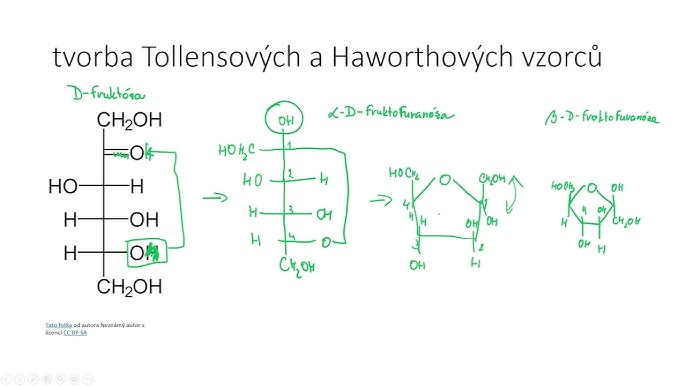
\includegraphics[width=\linewidth]{glukosa.png}
      \caption{}
  \end{figure}
  \item při tvorbě cyklického vzorce platí pravidlo: co je vlevo, bude nahoře -- když mám necykickou projekci tak skupiny připojené na uhlík, která jsou nalevo od něj píšu nahoru, ty napravo dolů (výjimkou je $CH_2OH$, které vždycky píšeme nahoru, ikdyž je vpravo), dále rozdělujeme $\alpha$ nebo $\beta$, alpha má na prvním uhlíku OH skupinu dole
\end{itemize}


\subsection{Redukující sacharidy}
\begin{itemize}
  \item aldosy mohou za pomocí redukčního činidla přejít do tzv. aldonové kyseliny, pro toto je potřeba, aby aldosa měla volnou hydroxy skupinu na anomerním uhlíku (na tom prvním)
  \item tedy vznikají deriváty sacharidů -- z karbonylové skupiny mám karboxylovou skupinu
  \item např. oxidací galaktosy vzniká kys. galaktonová, oxidací manosy vzniká kys. mannová
  \item při specifické oxidaci hydroxy-methylu na posledním uhlíku vznikají uronové kyseliny -- např. glukoronová kyselina
  \item sem patří i kys. L-askorbová -- výjimečná, že je L a ne D
  \begin{figure}[h]
      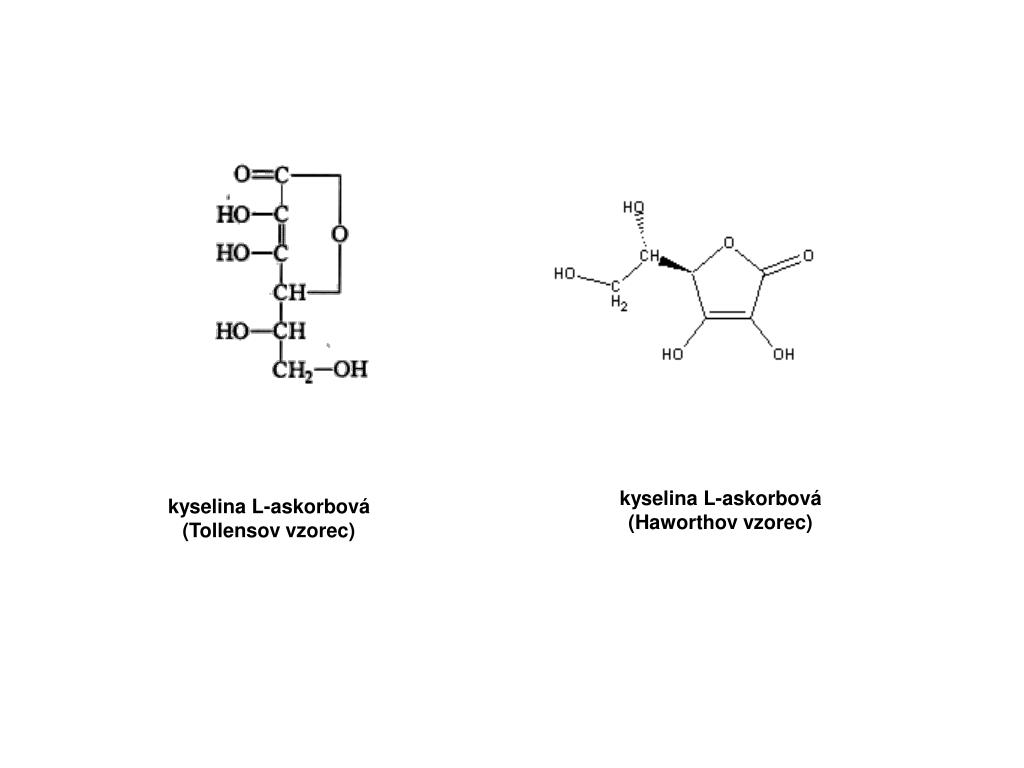
\includegraphics[width=\linewidth]{askorbova.png}
      \caption{}
  \end{figure}
  \item celulosa jsou dvě cyklické $\beta$-D-glukosy spojené $\beta$ 1,4 vazbou -- tzv. $\beta$-D-glukan (jsou tu jen glukosy, takže to takhle můžu nazvat)
  \item dále hemicelulosy -- něco dalšího k glukosam, např. arabany (v pektinových látkách), manany (celej rok jehličnan), xylany (nevim)
  \item  chitin -- dusíkatý derivát, hlavní jednotkou N-acetylglukosamin
  \item pektinové látky -- želírování, v ovoci, obsahuje kyselinu D-galakturonovou
  \item rostlinné zásobní polysacharidy -- škroby, především pětina amylosy (nevětvená, spirálovitá) a čtyři pětiny amylopektinu (větvená, síťovaná) -- obě dvě vybudovány z maltosových jednotek, škroby štěpeny $\alpha$-amylasou (sliny) a pankreatickou $\alpha$-amylasou (tenké střevo (pankreas)) a $\alpha$-glukosidasa, $\alpha$-dextrinasy a sacharasy (u malých dětí laktosa) (tlusté střevo)
  \item použití jako lepidla, impregnace textilu, kosmetika, jako srážedla (flokulanty -- zhušťovadla, zvločkovadla), dextriny
  \item alternativní sladidlo inulin
  \item zásobní polysacharid ve svalech a játrech -- celkově pro živočichy je glykogen -- glukosa spojena $\alpha$ 1,4 vazbami, větvený
  \item tukové buňky adipocyty -- buď hnědé (miminka) nebo bílé (dospělí)
  \item mukopolysacharidy -- převážně v pojivových tkáních jako mazadla nebo pojiva, většinou glukosaminy (mají dusík), např. kyselina hyaluronová -- schopna na sebe navázat hodně vody -- velmi dobře hydratuje -- využití v kosmetice (krémy, výplně), výskyt v bulvách, v kloubech
  \item mezi mukopolysacharidy patří třeba chondroitin-4-sulfát -- hlavní součást chrupavek, když se začne rozpadat tak přestane plnit svoji funkci -- osteoporosa
  \item heparin -- nachází se v tepenných buňkách, zabraňuje srážení krve -- inhibuje tvorbu faktorů, což znamená, že nemám katalyzátory toho srážení prostě
  \item glykoproteiny/proteoglykany -- sacharidová a proteinová složka, patří sem peptidoglykany -- buněčná stěna bakterií (dělení na gram-postiviní (silná stěna -- nezabarvené -- hůře léčitelné ATB) a gram-negativní (jednovrstevná stěna s kys. teichovou -- takže barvivo se nevymyje -- lépe léčitelné ATB)) (tohle je možná naopak btw)

\end{itemize}

\section{Lipidy}
\begin{itemize}
  \item látky nepolární podle starší definice jestli chápu správně, nevim novou definici
  \item dělí se na zmýdelnitelné (normální tuky) a nezmýdelnitelné (isopreny, terpeny)
  \item mastné kyseliny -- karbox. k. s uhlíkovým ocasem
  \item mastné kyseliny takové housneky, z nich se tvoří biomembrány
  \item nasycené -- tuhé (k. palmitová), nenasycené -- kapalné (k. olejová (18C 1=), linolová (18C 2=), linolenová (18C 3=))
  \item zápis: napíšu kolik je uhlíků před násobnou vazbu, napíšu násobnou vazbu, napíšu kolik je za násobnou vazbou, napíšu COOH, příklady: \\
  \begin{minipage}{0.5\textwidth}
      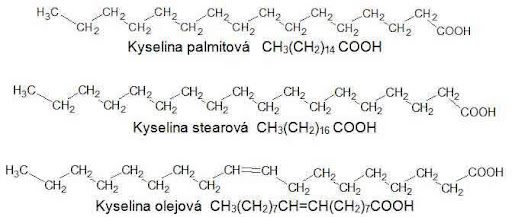
\includegraphics[width=\linewidth]{mastne_kyseliny.jpg}
  \end{minipage}
  \hfill
  \noindent\begin{minipage}{0.5\textwidth}
      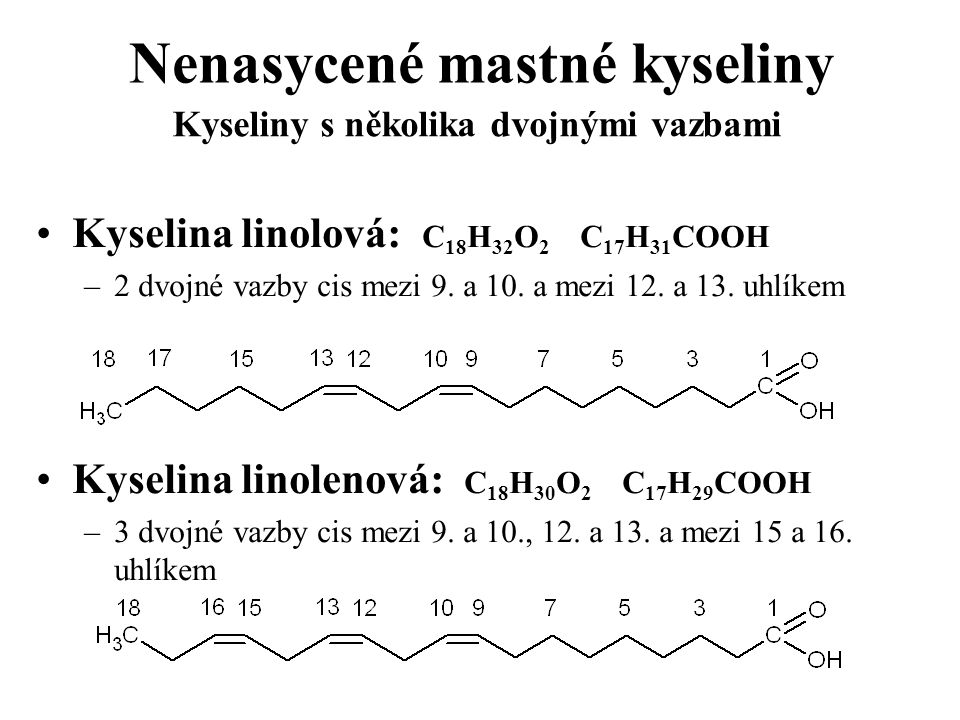
\includegraphics[width=\linewidth]{nenasycene_mastne_kyseliny.jpg}
  \end{minipage}
  \item triacylglyceroly -- tuky -- estery karbox. kys. -- glycerol se třemi ocásky mastných kyselin, hlavní zásoba, reakce esterifikace -- z glycerolu se odpojí H, z karbox. k. OH, a spojí se to dohromady, uhlíkové ocásky trčí ven
  \item metabolismem tuků získáme skoro 2x energie než sacharidů
  \item depotní (zásobní) tuk -- zdroje E na horší časy, pro tažné ptáky při hladovění, v rostlinách pro klíčení semen
  \item tuky krom zásob taky fce strukturní -- součástí membrán, nezbytné pro přenos vzruchů v NS
  \item taky ochranná fce -- v orgánech mazivo, obrana před mech. poškoz.
  \item lipidy jsou také vosky
  \item taky kutikula, lanolin
\end{itemize}
\subsubsection{složené lipidy}
\begin{itemize}
  \item pak jsou i složené lipidy, kde je i něco jiného kromě lkoholu a mastné kyseliny, často mají biologické fce
  \item např. fosfolipidy, které mají polární fosfátovou skupinu -- molekuly amfifilní
  \item nebo např. sfingolipidy -- deriváty sfingosinu, nachází se v membránách nervových buněk, zodpovědné za správný přenos vzruchů
  \item důležitý je taky cholesterol, je základem většiny pohlavních hormonů, také součástí biomembrán, HDL "špatný" cohlesterol, LDL "hodný"
  \item micela -- amfifilní molekula obklopí tuk a takto může být odnesen vodou -- čist. prostř.
\end{itemize}

\section{Enzymy}
\begin{itemize}
  \item biologické katalyzátory
  \item urychlují reakce lépe než anorganické
  \item více specifické, regulovatelné koncentrací jiných látek kromě substrátu
  \item S (substrát) + E (enzym) $\rightarrow$ [ES] $\rightarrow$ [EP] $\rightarrow$ E + P'
  \item koncovka -asa (mam X a X štěpí X-asa)
\end{itemize}
Druhy enzymů
\begin{itemize}
  \item oxidoreduktasy
  \item transferasy
  \item hydrolysy
  \item ...
  \item ligasy
  \begin{itemize}
    \item katalyzují vznik vazeb za užití ATP
    \item např pyruvátkarboxylasa katalytuje zabudování CO2 do pyruvátu za vzniku oxalacetátu
  \end{itemize}
\end{itemize}
Struktura enzymů
\begin{itemize}
  \item jednosložkové enzymy -- pouze z bílkovin
  \item dvousložkové enzymy -- mají nebílkovinnou část apoenzym + kofaktor = holoenzym
\end{itemize}
Kofaktory
\begin{itemize}
  \item koenzymy -- nejsou pevně připojeny k enzymu a mohou tak disociovat
  \item prostetické skupiny -- jsou pevně připojeny
\end{itemize}
\begin{figure}[h]
    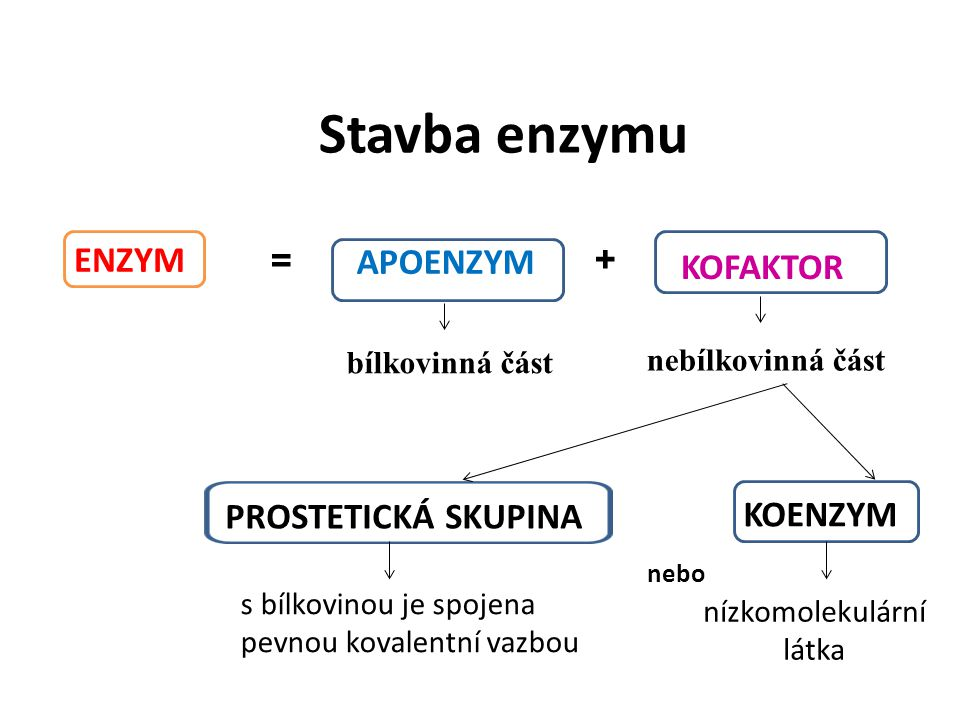
\includegraphics[width=0.5\linewidth]{stavba_enzymu.jpg}
\end{figure}
\begin{itemize}
  \item každý enzym má tzv. aktivní místo -- tvarově (stericky) to je doplněk k substrátu, takže ho zachytavá
\end{itemize}
Výskyt a forma enzymů
\begin{itemize}
  \item podle místa výskytu
  \begin{itemize}
    \item intracelulární -- většina, buď v rozpuštěné formě, nebo vazané v strukturách -- multienzymových komplexech
    \item extracelulární -- z buněk vylučovány
  \end{itemize}
  \item specificita enzymů
  \begin{itemize}
    \item učinková -- k typu reakce, tentýž substrát může být přeměňován několika enzymy na různé produkty
    \item substrátová
    \begin{itemize}
      \item absolutní -- přeměňuje jen jeden specificky substrát
      \item skupinová -- přeměňuje skupinu substrátu téhož typu
      \item relativní skupinová -- přednostně katalyzuje reakce stejné skupiny, je však schopen ve zmenšené aktivitě působit na jiné substráty
    \end{itemize}
  \end{itemize}
\end{itemize}
Mechanismus účinku enzymů
\begin{itemize}
  \item teorie komplementarity (teorie klíče (substrát) a zámku (enzym))
  \item
\end{itemize}

zase tady něco není sdhfiosdg

Inhibice
\begin{itemize}
  \item inhibitory -- látky, které snižují aktivitu enzymu
  \item rozlišujeme několik druhů
  \begin{itemize}
    \item kompetetivní
    \begin{itemize}
      \item inhibitor soutěží s molekulou substrátu o vazbu v aktivním místě -- vytěsňuje substrát, inhibitor se naváže místo něho, reakce neprobíhá
    \end{itemize}
    \item akompetetivní
    \begin{itemize}
      \item inhibitor se neváže na enzym, ale na komplex enzym-substrát, navázání inhibitoru vyvolá strukturní změny v enzymu, takže se nestane žádná reakce
    \end{itemize}
    \item allosterická
    \begin{itemize}
      \item inhibitor se naváže na jiné než aktivní místo enzymu, tím způsobí v aktivním místě změnu konformace, takže se zde nemůže navázat substrát
    \end{itemize}
  \end{itemize}
  \item existuje také inhibice substrátem a produktem reakce -- pokud je substrát ve velkém nadbytku $\rightarrow$ substrát se na enzym napojí na více místech a přestává tak fungovat, dojde ke zpomalení až zastavení reakce
\end{itemize}

\subsection{Hormony}
\begin{itemize}
  \item sloučeniny, které slouží v těle jako chemický posel od jdné buňky pro jiné
  \item řídí průběh a vzájemnou koordinaci reakcí v organismu
  \item od enzymů se liší tím, že působí pouze na žijící buňky
  \item podle vzdálenosti působnosti
  \begin{itemize}
    \item autokrinní -- působí na buňku, která je uvolnila
    \item parakrinní -- působí na buňky blízké té, která je uvolnila
    \item endokrinní -- působí po celém těle
    \item feromony -- působí na jedince téhož druhu, většinou jako sexuální lákadlo
  \end{itemize}
  \item některé důležité hormony
  \begin{itemize}
    \item
  \end{itemize}
\end{itemize}

\subsubsection{Receptory}
\begin{itemize}
  \item místa, která reagují na signální molekuly hormonu
  \item můžou se rozlišovat podle místa kde vážou sign. molekuly -- cytoplasmatické, jaderné, transmembránové
\end{itemize}

\subsection{Vitaminy}
\begin{itemize}
  \item důležitý koenzym (peptid, polysacharid)
  \item zabraňují třeba oxidaci v tkáni
  \item většinu musíme přijímat ve stravě -- nedokážeme si vyrobit sami
  \item rozpustné v tucích (A, D, E, K) x rozpustné ve vodě (B, C)
  \item
\end{itemize}

\end{document}
